\section{Zagadnienia Kontrolne}
\begin{enumerate}
    \item \par{Prawo Hooke'a - odkształcenie ciała pod wpływem, działającej siły jest proporcjonalne do tej siły. Współczynnik między naprężeniem wywołanym przez przyłożone siły odkształceniem nazywany jest modułem Young'a. Prawdziwe dla niedużych odkształceń i~tylko dla niektórych materiałów o ~pomijanie małej plastyczności. Można je wyrazić  wzorem:
    \[\frac{F}{S}=E\frac{\Delta L}{L}\]}
    \begin{itemize}
        \item[ ] $\Delta L$ - różnica długości
        \item[ ]  $L$ - pierwotna długość
        \item[ ]  $E$ - moduł Young'a
        \item[ ]  $S$ - powierzchnia przekroju poprzecznego
        \item[ ]  $F$ - siła działająca na ciało
    \end{itemize}
    Odkształcenie sprężyste - rodzaj odkształcenia, które ustępuje po usunięciu siły wywołującej to odkształcenie 
    \addtocounter{enumi}{1}
    \addtocounter{enumi}{1}
    
    \item Moduł Younga - wielkość opisująca sprężystość materiału przy pościąganiu i ściskaniu. Wyraża ona zależność względnego odkształcenia materiału do naprężenia jakie wnim występuje w zakresie odkształceń sprężystych wyraża się je w Pascalach $E=\left[\frac{N}{m^2}\right]=[\text{Pa}]$ 
    
    \item Co się stanie z Drutem po przekroczeniu jego granicy sprężystości?
    
    Po przekroczeniu granicy sprężystości rozpocznie się nieodwracalne odkształcenie drutu tj. po usunięciu siły działającej na drut pozostanie on trwale odkształcony.
    
    \item Dlaczego zmiany długości drutu s 2razy mniejsze od zmian długości  podawanych przez czujnik?
    Zmiany długości drutu ($d$) są 2 krotnie mniejsze od długości podawanej przez czujnik $D$, ponieważ są przyprostokątnymi dwóch trójkątów podobnych, których skala podobieństwa $k=\frac{A}{a}=2$, z powodu umiejscowienia drutu w połowie długości ramienia dźwigni.
    
    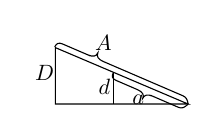
\begin{tikzpicture}[x=0.75pt,y=0.75pt,yscale=-0.4,xscale=0.4]
%uncomment if require: \path (0,446.25); %set diagram left start at 0, and has height of 446.25

%Straight Lines [id:da9313950171592851] 
\draw (430,100) --(270,32) -- (270,100)--(430,100)--(270,32)  ;


%Straight Lines [id:da6902289836929021] 
\draw (340,62) -- (340,100) ;
 ;


%Shape: Brace [id:dp7000132748697048] 
\draw   (430,100) .. controls (429.13,94.91) and (427.91,91.85) .. (423.62,90) -- (327.65,48.69) .. controls (321.53,46.06) and (319.39,42.6) .. (321.24,38.31) .. controls (319.39,42.6) and (315.41,43.42) .. (309.28,40.78)(312.04,41.97) -- (278.49,27.53) .. controls (274.2,25.68) and (271.14,26.9) .. (269.29,31.19) ;
%Shape: Brace [id:dp41634221637891644] 
\draw   (340,62) .. controls (337.43,66.49) and (338.65,69.55) .. (342.93,71.4) -- (368.93,82.63) .. controls (375.05,85.28) and (377.19,88.74) .. (375.34,93.02) .. controls (377.19,88.74) and (381.17,87.92) .. (387.29,90.56)(384.54,89.37) -- (418.08,103.86) .. controls (422.36,105.71) and (425.43,104.49) .. (430,100) ;


% Text Node
\draw (257,62) node [scale=0.8  ,opacity=1 ]  {$D$};
% Text Node
\draw (328,26) node [scale=0.8  ,opacity=1 ]  {$A$};
% Text Node
\draw (370,95) node [scale=0.8  ,opacity=1 ]  {$a$};
% Text Node
\draw (329,79) node [scale=0.8  ,opacity=1 ]  {$d$};

\end{tikzpicture}
%\pagebreak
\item Czym różni się definicyjny wzór na moduł Younga od wzoru roboczego:

Wzór definicyjny na moduł Younga:
\[E=\frac{\sigma}{\varepsilon} = \frac{\frac{F}{S}}{\frac{\Delta L}{L}} = \frac{FL}{S\Delta L}\]
Natomiast Wzór roboczy ma formę:
\[E=\frac{4L}{\pi d^2a} = \frac{L}{Sa}\]
gdzie $a$ jest współczynnikiem nachylenia prostej wyrażającej zależność $\Delta L(F)$, która z prawa Hooka powinna być linią prostą.
\end{enumerate}